% Chapters
%!TEX root = ../report.tex
\chapter{Sprint Planning}\label{chap:s4_sprintplanning}
This sprint planning proceed ordinarily as specified by the development method. We first have a sprint planning in the subproject followed by sprint planning in the group.

\begin{chapterorganization}
  \item in \sectionref{sec:S4_bd} we describe the user stories we commit ourselves to during the \bd sprint planning meeting.
  \item in \sectionref{sec:S4_group} we describe the sprint planning in our group and lists our tasks with reference to a backlog item.
\end{chapterorganization}

\section{\bdtitle Sprint Planning}\label{sec:S4_bd}
During the \bd sprint planning we choose to work on four user stories and one technical work item. They are labeled with a number in parentheses for reference. In the last sprint we specified precisely the backlog items used and how to formulate user stories (see \sectionref{sec:processspecs}).

Each user story now has a number of \emph{conditions of satisfaction}. These conditions of satisfaction are listed as bullets below each user story. The conditions have been elicited by asking our customers and our product owner.

\begin{description}
  \item[(1)] As a developer I want libraries to have higher priority than other jobs in the build scheduling on Jenkins so that libraries are not bottlenecked when several people are reliant on them.
  \begin{itemize}
    \item Jobs must not be starved
    \item Libraries must be prioritized higher than other job types
  \end{itemize}
  \item[(2)] As a developer I want tests to run on the debug version of apps so that they can be tested on a test database.
  \begin{itemize}
    \item Monkey tests must run on debug APKs
  \end{itemize}
  \item[(3)] As a developer I want an easy way to download and install all apps so that it is easy to test the apps combined, and easy to show the external customers.
  \begin{itemize}
    \item Users should not have to install additional software onto their computers
    \item Users should be able to merely run a program that then automatically downloads and installs all apps on a device
    \item After running the program, the device must contain the newest version of all apps
  \end{itemize}
  \item[(4)] As a future developer I want to know what is on Jenkins and how it is structured so that it it is easy to start working with
  \begin{itemize}
    \item Document how to configure projects
    \item Document configuration of authentication
    \item Document files used for automation
  \end{itemize}
  \item[(5)] As a developer I want to have a screenshot taken when a monkey test fails so that I can get feedback about the failure
  \begin{itemize}
    \item The last screen at a crash must be saved
  \end{itemize}
\end{description}

The following is the technical work item we work on in sprint 4. This technical work item is not formulated as a user story, as it is hard to have conditions of satisfaction for it. The build time can almost always be decreased, and so it would be a never-ending user story. We choose to work on it in this sprint, as it was prioritized highly by the other groups, as there are still improvements to be made, mostly related to the emulator.

\begin{description}
  \item[(6) Decrease Job Build Times on Jenkins] When the queue on Jenkins is long, jobs can take a very long time to build. As we discussed in \sectionref{sec:non-emulator_testing}, the build times can be further reduces by working on the emulator.
\end{description}

\section{Group Sprint Planning}\label{sec:S4_group}
At our internal sprint planning we divide the chosen backlog items into tasks and estimate them. For this sprint, we have a total of 70 half days of work. \tableref{tab:sprint4_tasks} shows the tasks we have committed to solve for this sprint. Tasks with a plus (+) are tasks that have been added during the sprint as they were discovered. Tasks with an estimation of 0 have been estimated as such, because they take virtually no time. There are three tasks in the sprint backlog which are not directly related to any backlog item. We do these because 

In addition to the tasks related to solving our chosen backlog items, we also work on report related tasks to finish our report, such as introduction, conclusion, etc. The total amount of time estimated for report tasks during this sprint is 56.

The total estimate for the original tasks is quite low (18). This is because we do a number of spikes, as indicated in parentheses for those tasks. We do these spikes because we have many uncertainties during this sprint. The final total estimate is therefore 37. The estimation for all tasks (report and non-report tasks) is 93. This far exceeds the time we have available for this sprint. Since we have a week following the sprint to do the final report changes, we postpone some report tasks. We therefore only manage to make 36 units of report tasks during this sprint, missing 20 units. The total amount of achieved work this sprint is therefore 73.

\begin{table}%
  \centering
  \begin{tabular}{p{0.6\textwidth}rr}
    \toprule
    \textbf{Task} & \textbf{Backlog Item} & \textbf{Estimation} \\
    \midrule
    Investigate conditions of satisfaction for our back log items & na & 2 \\
    Check monkey tests after server crash (+) & na & 2 \\
    Make pre-commit hook (+) & na & 1 \\
    Install Jenkins priority plugin & 1 & 1 \\
    Choose schedule method for priority plugin & 1 & 2 \\
    Give metadata high priority (+) & 1 & 0 \\
    Make monkey tests use debug APKs & 2 & 1 \\
    Place debug APKs in a specific directory & 2 & 1 \\
    Make script for downloading and installing newest APKs & 3 & 2 \\
    Identify areas for Jenkins structure documentation (spike) & 4 & 2 \\
    Write about Jenkins structure & 4 & 2 \\
    Write about Jenkins files & 4 & 2 \\
    Make monkey tests take screenshot and publish them & 5 & 0 \\
    Make ADB-wifi app (+) & 6 & 2 \\
    Setup Jenkins Job for Simiasque (+) & 6 & 1 \\
    Investigate usage of physical tablets (spike) & 6 & 1 \\
    Run monkey test without emulator plugin (+) & 6 & 2 \\
    How do we automatically connect to tablets? (spike) & 6 & 2 \\
    Connect to all devices wirelessly from server (+) & 6 & 2 \\
    Uninstall APKs on all devices (+) & 6 & 1 \\
    Setup router (+) & 6 & 2 \\
    Only start an emulator when there are no connected devices (+) & 6 & 6 \\
    \midrule
    \textbf{Original total} & & 18 \\
    \textbf{Total} & & 37 \\
    \bottomrule
  \end{tabular}
\caption[Sprint 4 backlog]{Sprint backlog for sprint 4, excluding report tasks. The tasks are listed in no particular order.}
\label{tab:sprint4_tasks}
\end{table}

\section{Upload of Apps to Google Play}\label{sec:upload_google_play}
Jenkins compiles and builds the Giraf projects but does nothing with the generated APKs. One of the user stories selected in this sprint is \us{automatic upload of alpha releases to Google Play}.

Before the APKs can be published to Google Play, they need to be signed with a signature. The Android plugin for Gradle has functionality for automatic signing of APKs, and we will use this to sign. A keystore file is used to sign, and we are not interested in everybody having this file as it serves as a proof of identification. We save the file on the server, which means that it becomes impossible to build release versions of the apps locally using the Giraf keystore. When uploading a new app to Google Play, the version code of the new app must be greater than the version code of the app already in the app store. Incrementing the version code is not done per default, so we need to set up the build to increase the version code every time an app is successfully built. 

We have written a Gradle plugin handling this with the major part of this seen in \listingref{lst:gradle_versioncode}. The plugin keeps a properties file with the current version code for all apps. Upon executing the \mono{increaseVersionCode} Gradle task, it reads the version code (line 8) from the properties file and increments it (line 12). Then it writes it to the app manifest file (line 13), such that the build following will use the new version code. Finally, it updates the property file with the new version code (line 15), such that the next build will use this version code. If no current version code is found in the properties file (line 21), we assume the app is new and starts at version code \mono{1}, and as such we do not increment it (line 10).
\begin{gradlecode}[caption=Part of our Gradle plugin for updating version code,label=lst:gradle_versioncode]
project.task('increaseVersionCode') << {
    // [...]
    // Check to see if properties file exists.
    if (project.file(versionCodesFilePath).exists() != true) {
        throw new GradleException("No version code file found. Only Jenkins should run this task")
    }
    // [...]
    def newVersion = getVersionCode(project, applicationId)
    def versionCode = newVersion['value']
    if (!newVersion['created']) {
        // Increment version code if not new
        versionCode++
        // Write incremented version code to manifest
        // [...]
        // Write incremented version code back to properties file
        // [...]
    }
}

def getVersionCode(project, applicationId) {
    // Reads the version code from the properties file. Returns 1 if the version code does not exist.
}
\end{gradlecode}
 
Now that the APKs have been signed, they need to be uploaded to Google Play. This can be done in two ways: Via a Jenkins plugin \parencite{jenkins-play-plugin} or through Gradle \parencite{gradle-play-plugin}. The Jenkins plugin is easy to use, but requires that the exact name and location of the of the APK to upload is known. The Gradle plugin knows this already, since the information is already present in the Gradle build environment. Therefore we use Gradle to publish to Google Play via a Google Play API\@. After the APKs have been uploaded, they are moved to the ftp server which is hosted on the same machine as Jenkins in the directory \mono{/srv/ftp/}. This way the APKs are also available outside of the Google Play store.

\chapter{Restructuring of Jenkins}
The setup of Jenkins used in sprint 0 was tedious to work with since all jobs were configured independently. If a change had to be made to several jobs, we would have to manually configure the change in each job. Not only did this take a considerable amount of time, but it was also prone to human errors during the process. We install a Jenkins plugin which allows jobs to have inheritable properties. As such, when we decide to make a change to e.g.\ the build system, it will not be necessary to change this in each job. Instead, the change can be made one place, and since all relevant jobs inherit they will inherit this change. This also ensures that jobs follow a consistent pipeline and thus do not differ in from job to job.

We find that almost all jobs on Jenkins will benefit from this, and we see two general categories that are sufficiently distinct: Android apps and Android libraries. We create an abstract job for each of these. They do overlap somewhat in functionality, which means we have to create an abstract job for each job task. As such we create abstract jobs for e.g.\ \emph{run Gradle}, \emph{run unit tests}, \emph{find and move APKs}, and \emph{publish lint report}. The abstract jobs \emph{Android app} and \emph{Android library} inherit from the small abstract tasks that are relevant.

Doing this also means we have to recreate all jobs, and a result of this is that the build history of each job is lost. We do not consider this a major problem, since most of the projects at this point do not build anyway.

We have modelled this as an OOP class diagram in \todo{Pæn graf over Jenkins jobs og inheritance?}

\todo{Nævn at vi ikke har en specifik user story for this. Det er refaktorering}

\chapter{Some Chapter}
\section{Improving Build Times}

To identify in which parts of the build process to make faster, we measure the time different parts of the Launcher project take. The Launcher project is the main application which depends on many other subprojects. The timings are measured on the Jenkins server and shown in \figureref{fig:launcher_build_times}. The shows the build timings of the Launcher application and the different subprojects (\emph{Oasis-lib, Giraf-Component, Local-db, Barcode-scanner, and Metadata}), as well as the startup time for the emulator.\todo{Kan vi regne med, at submoduler bliver binære filer?}

\begin{figure}
\centering
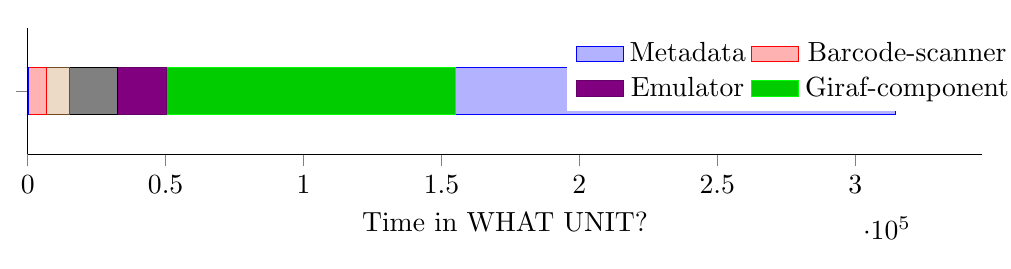
\begin{tikzpicture}[trim axis left, trim axis right]
  \begin{axis}[
    xbar stacked,
    scale only axis,
    width=\textwidth,
    axis y line*= none, axis x line*= bottom,
    %xmajorgrids = true,
    ytick = data,
    yticklabels = {},
    tick align = outside,
    %xtick pos = left,
    bar width=6mm,
    y=8mm,
    %nodes near coords,
    legend style={
      legend columns=4,
      anchor=north,
      yshift=0ex,
      xshift=0ex,
      draw=none
      %legend cell align=left
    },
    area legend,
    xlabel = {Time in WHAT UNIT?},
    xmin = 0
  ]
    \addplot coordinates
    {(209,0)}; 
    \addlegendentry{Metadata}
    \addplot coordinates
    {(6625,0)};
    \addlegendentry{Barcode-scanner}
    \addplot coordinates
    {(8393,0)};
    \addlegendentry{Launcher}
    \addplot coordinates
    {(17223,0)};
    \addlegendentry{Local-db}
    \addplot coordinates
    {(18000,0)};
    \addlegendentry{Emulator}
    \addplot coordinates
    {(104696,0)};
    \addlegendentry{Giraf-component}
    \addplot coordinates
    {(159497,0)};
    \addlegendentry{Oasis-lib}
    %\legend{Test, test, test, test, test, test}
  \end{axis}
\end{tikzpicture}
\caption{Timings during build of the Launcher project.}\label{fig:launcher_build_times}
\end{figure}

\chapter{Sprint Two Review}\label{chap:sprint2_end}

\begin{chapterorganization}
  \item in \sectionref{sec:s2_goals} we \todo{fill out};
  \item in \sectionref{sec:s2_multiprj_review} we \todo{fill out}.
\end{chapterorganization}

\section{Sprint Goals}\label{sec:s2_goals}
\todo{Monkey test tog en del længere tid end estimeret.}

\todo{Vi droppede at kigge videre på at forbedre emulator speed fordi vi fokuserede på at fjerne build times på submodules. Der kom nogle nye tasks til, og vi reducerede derfor kraftigt tiden på de tasks der kiggede på emulatorforbedringer.}

\todo{Vi havde ikke nok tid til at skrive rapport for dette sprint. Vi brugte også noget tid på at færdiggøre rapport fra sidste sprint. Estimering på dette var en smule større end faktisk brugt, men passede ellers rimelig godt.}

\section{Multi-Project Sprint Review}\label{sec:s2_multiprj_review}
Again, a common meeting among all groups is held to evaluate and reflect upon the process in this sprint.

It was noticed that chickens during the meetings of this sprint had been too noisy at times. We pointed out that chickens should find alternative means of communicating during meetings, and hope this will be enough. Otherwise, we will point it out during meetings.

Also, some groups repeatedly did not show up to sprint meetings. We decided to find out the reasons behind it, knowing we cannot force them to show up. One group responded that they simply forgot the meetings, but will be more careful of remembering meetings in the future.

Two days between the \gui and the other two sprint planning meetings, suggested at the sprint 1 multi-project review, was implemented in this sprint. The feedback was positive and people were happy with this approach. As such we continue with it.

A suggestion was made allowing a product owner from \db and \bd to participate as pigs in the \gui sprint planning meeting. This seems like a good idea as they may have some useful input. We will add this to the development method.

It was suggested to add a feature freeze, but was quickly dismissed. Instead, we pleaded people to use common sense regarding implementing last minute changes before a sprint end. We also reminded people that they should talk to affected groups before making a change.
